Do zaimplementowania aplikacji internetowej wykorzystane zostały biblioteka React oraz framework
Next.js. Oba wykorzystywane są do budowania interaktywnych interfejsów użytkownika. React jest
biblioteką deklaratywną -- oznacza to, że podczas pisania kodu źródłowego dla aplikacji opisuje się
warunki jakie dany element interfejsu powinien spełniać~w~przeciwieństwie do podejścia
imperatywnego, gdzie podaje się szczegółową listę kroków prowadzących do osiągnięcia założonego celu
\cite{react-main}. Next.js jest frameworkiem zbudowanym na podstawie React.
Zapewnia środowisko~z~funkcjami do tworzenia aplikacji: renderowanie hybrydowe -- opierające się na
wstępnym wygenerowaniu elementów aplikacji~i~następnie aktualizowanie ich~w~miarę potrzeb,
inteligentne łączenie kodu źródłowego~w~pakiety, wstępne ładowanie tras (które łączą różne elementy
aplikacji), wszystko to zapewnione jest bez uprzedniej, dodatkowej konfiguracji \cite{nextjs-main}.

Dodatkowo wykorzystane zostały biblioteki pomocnicze, które przyspieszały~i~znacznie
ułatwiały budowanie interfejsu użytkownika. Wykorzystana biblioteka Chakra UI daje dostęp do wielu
gotowych, wystylizowanych komponentów, które można,~w~miarę potrzeb dostosować, aby efekt końcowy
był jak najbliższy projektowi. Wykorzystane zostały także biblioteki React Latex oraz Recharts.
Pierwsza pozwala na renderowanie formuł matematycznych~w~aplikacji, używając do tego zapisu
znanego~z~pakietu LaTeX, druga natomiast służy do generowania wykresów, które pojawiają
się~w~aplikacji. Wszystkie wykorzystane biblioteki oraz frameworki należą do rodziny Open Source --
ich kod źródłowy jest dostępny publicznie, można go wykorzystywać~i~modyfikować~w~swoich
projektach, zgodnie~z~opublikowaną licencją \cite{snyk-licences, snyk-mit}.

Aplikacja została zaimplementowana wykorzystując do tego język TypeScript. Jest on nadzbiorem --
rozszerzeniem -- języka JavaScript. TypeScript umożliwia statyczne typowanie oraz programowanie
obiektowe, gdzie JavaScript jest językiem skryptowym. Wykorzystanie TypeScript~w~programowaniu
pozwala na unikanie błędów, które~w~późniejszym czasie mogłyby doprowadzić do nieplanowanego
zachowania tworzonej aplikacji. Aplikacje, napisane~w~TypeScript, są interpretowane oraz
kompilowane do JavaScript, aby można było je uruchomić przykładowo~w~przeglądarce
internetowej \cite{ts-main}.

Niniejszy rozdział ma na celu:
\begin{itemize}
      \item[--] przedstawienie jak zbudowane zostały główne elementy interfejsu użytkownika,
      \item[--] pokazanie jak odbywa się konfiguracja elementów aplikacji oraz zarządzanie stanem
            komponentów,
      \item[--] zaprezentowanie, że kod odpowiedzialny za generowanie danych oraz weryfikację ich
            jest zaimplementowany na podstawie teorii przetworników pomiarowych.
\end{itemize}

\section{Implementacja interfejsu użytkownika}\label{sect:ui}
% Opisanie tego jak zbudowane jest UI ogólnie, nawiązanie, że opisane zostaną tylko te najważniejsze
Całość kodu źródłowego aplikacji, która odpowiedzialna jest za renderowanie interfejsu użytkownika
wykorzystuje paradygmat programowania komponentowego -- pozwala na projektowanie, implementację oraz
testowanie elementów aplikacji niezależnie od siebie. Dodatkowo, jeżeli zaistnieje taka potrzeba,
część kodu źródłowego może być stworzona~w~zupełnie innym języku programowania, a~następnie
dołączona do aplikacji, gdzie będzie idealnie współpracować~z~resztą obecnych już komponentów
\cite{component-programming}. Interfejs użytkownika~w~aplikacji jest~w~języku angielskim. Został
stworzony~w~taki sposób, aby finalna aplikacja mogła być wykorzystywana przez użytkowników nie
tylko~z~Polski.

% Opis poszególnych, ważnych składowych UI ze snippetami
\subsection{Elementy interfejsu}
Głównymi elementami interfejsu są komponenty odpowiedzialne za:
\begin{itemize}
  \item[--] konfigurację sensora dla danego laboratorium,
  \item[--] wyświetlanie zadań do wykonania oraz wygenerowanych danych,
  \item[--] przyjmowanie oraz weryfikowanie odpowiedzi wpisywanych przez użytkownika,
  \item[--] prezentowanie wzorów oraz danych niezbędnych do obliczeń,
  \item[--] wyświetlanie wygenerowanego wykresu.
\end{itemize}
Powyższe elementy przedstawione zostały na rysunkach \ref{img:config-tasks},
\ref{img:generated-graph}, \ref{img:theory}.

\begingroup
\begin{figure}[!htb]
  \centering
  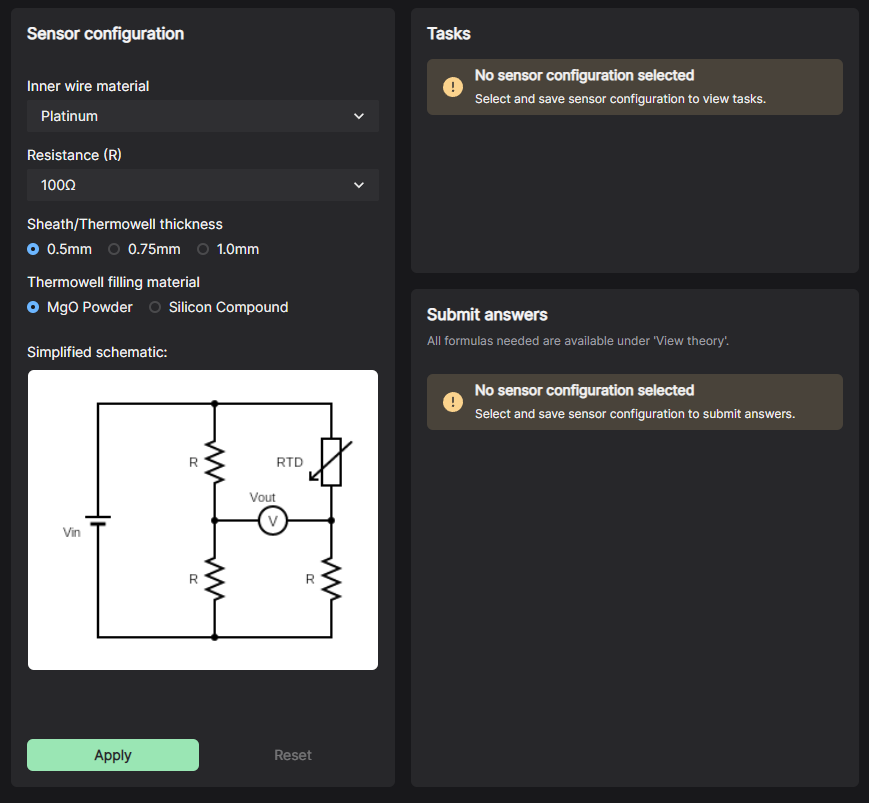
\includegraphics[width=0.65\textwidth]{app-ui/config-tasks}
  \caption{\label{img:config-tasks}Komponenty do konfiguracji, wyświetlania zadań~i~przyjmowania
    odpowiedzi.}
\end{figure}

\begin{figure}[!htb]
  \centering
  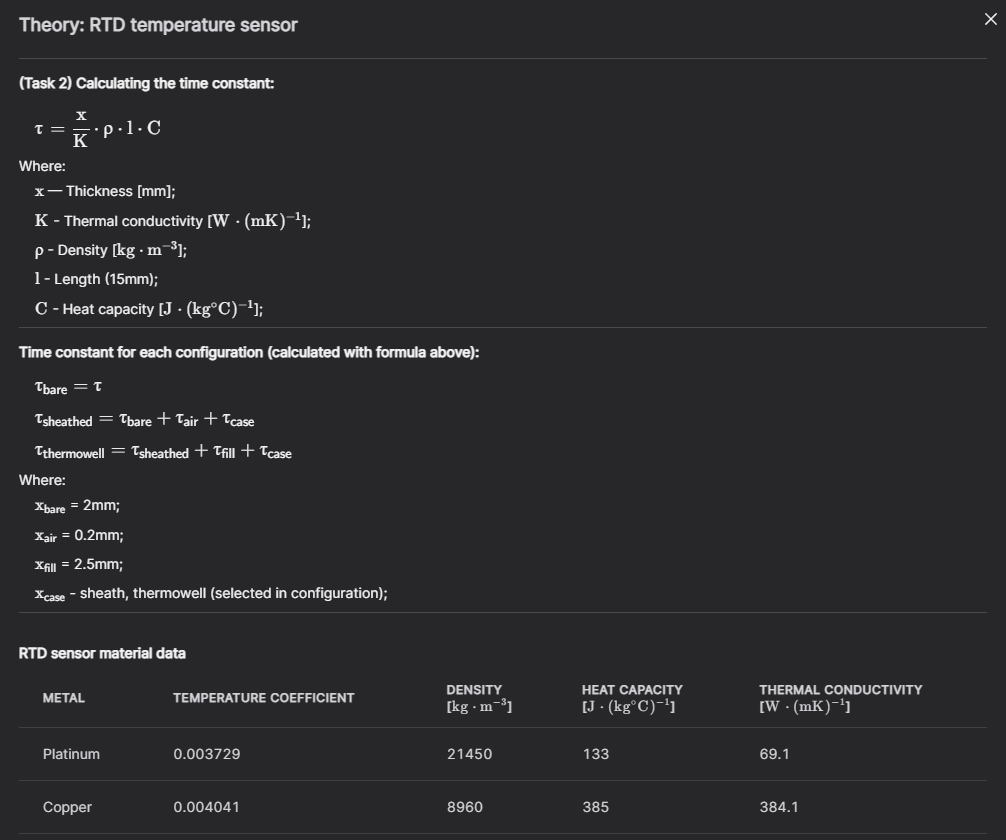
\includegraphics[width=0.65\textwidth]{app-ui/theory}
  \caption{\label{img:theory}Komponent prezentujący wzory oraz dane.}
\end{figure}

\begin{figure}[!htb]
  \centering
  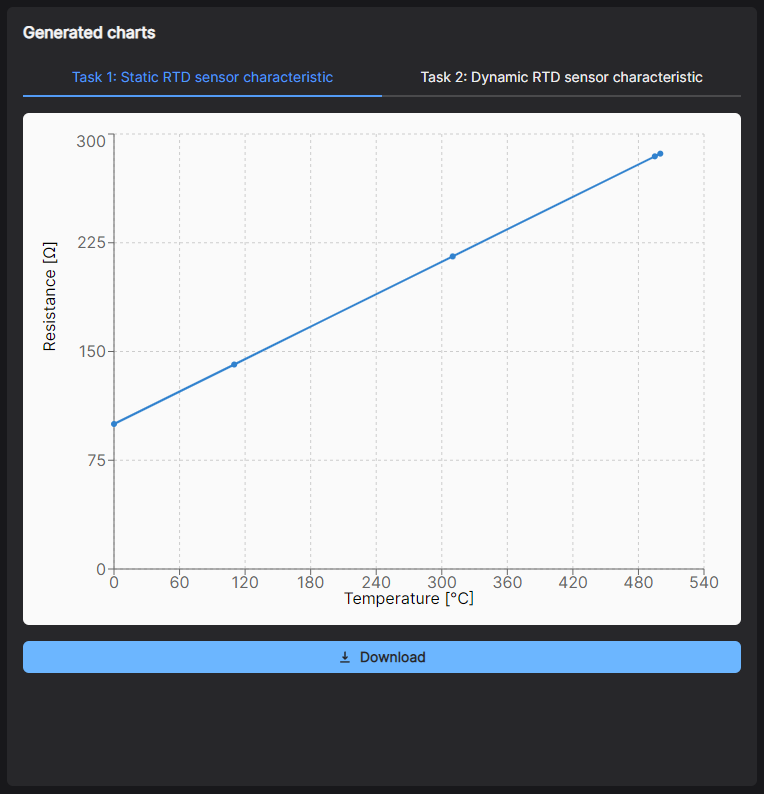
\includegraphics[width=0.65\textwidth]{app-ui/generated-graph}
  \caption{\label{img:generated-graph}Komponent wyświetlający wygenerowany wykres.}
\end{figure}
\endgroup

\subsubsection{Komponent do konfiguracji sensorów}
Dla każdego sensora możliwa jest zmiana jego parametrów. Do implementacji wykorzystana została
metoda dynamicznego mapowania pól~w~całym komponencie na podstawie pliku konfiguracyjnego,
odpowiadający za to kod przedstawiony został na rysunku \ref{lst:config-field-map}. Dane pole
posiada dwa różne warianty do wyboru -- wybór~z~listy (wykorzystywany~w~przypadkach, gdy dany
parametr ma więcej opcji do wyboru) lub przycisk typu radio (dla przypadków, gdzie opcji do wyboru
jest nie więcej jak trzy). Na rysunku \ref{lst:config-field} przedstawiony został kod, który
renderuje pojedyncze pole na podstawie informacji zawartych~w~pliku konfiguracyjnego, którego
fragment przedstawiony został na rysunku \ref{lst:config-field-data}.

\addimage{0.9}{code/config-field-map}{\label{lst:config-field-map}Funkcja dynamicznie mapująca pola
  na podstawie pliku konfiguracyjnego}

\addimage{0.9}{code/config-field}{\label{lst:config-field}Kod komponentu pojedynczego pola
  konfiguracyjnego}

\addimage{0.9}{code/config-field-data}{\label{lst:config-field-data}Fragment pliku zawierającego
  dane do generowania pól konfiguracyjnych}

Plik konfiguracyjny ma formę tablicy zawierającej obiekty, które definują dane pole. Każdy obiekt
składa się~z~par klucz-wartość. Klucz \colortt{sensor} określa do jakiego laboratorium przynależą
definiowane wartości, \colortt{id} wykorzystywany jest przy manipulowaniu stanem, którego zadaniem
jest przechowywanie informacji~o~obecnej konfiguracji sensora, natomiast \colortt{type} pozwala na
zdefiniowanie jaki wariant pola konfiguracyjnego ma zostać wyświetlony. Zarządzanie stanem oraz jak
zostało to rozwiązane~w~aplikacji opisane zostało~w~rozdziale \ref{sect:context}. Pozostałe klucze
-- \colortt{label, options, optionLabels, defaultValue} wykorzystywane są do określenia
wyświetlanego tytułu pola konfiguracyjnego, opcji dostępnych do wyboru oraz domyślnie
wybranej opcji.

\subsubsection{Komponent wyświetlający zadania oraz wygenerowany zestaw danych}
\lipsum[1]


\subsubsection{Komponent odpowiedzialny za przyjmowanie i weryfikację odpowiedzi}
\lipsum[1]


\subsubsection{Komponent prezentujący wzory oraz dane niezbędne do obliczeń}
Część teoretyczna do każdego laboratorium prezentowana jest~w~postaci okna dialogowego. Taka
implementacja została wykorzystana, aby użytkownik nie musiał zamykać strony~z~wykonywanym
ćwiczeniem (co skutkowałoby utratą postępów, ponieważ aplikacja nie posiada bazy danych). Zawartość
okna dialogowego konfigurowana jest przez dwa dodatkowe komponenty -- \texttt{Formula, Table},
których zadaniem jest generowanie odpowiednio listy wzorów oraz tabel~z~danymi na podstawie plików
konfiguracyjnych. Kod źródłowy odpowiadający za generowanie listy wzorów oraz tabel przedstawiony
jest~w~listingach \ref{lst:theory-formula} oraz \ref{lst:theory-table}, natomiast~w~listingach
\ref{lst:formula-config}, \ref{lst:table-config} przedstawione zostały fragmenty plików, które
zawierają informacje jakie wzory oraz tabele mają zostać wygenerowane przez komponenty.

\addsnippet{0.9}{code/theory-formula}{\label{lst:theory-formula}Kod komponentu odpowiedzialnego za
  generowanie listy wzorów}

\addsnippet{0.9}{code/theory-table}{\label{lst:theory-table}Komponent generujący tabele~z~danymi do
  ćwiczenia~w~oknie dialogowym}

\addsnippet{0.9}{code/formula-config}{\label{lst:formula-config}Fragment pliku~z~informacjami o
  wzorach do wyświetlenia~w~oknie dialogowym}

\addsnippet{0.9}{code/table-config}{\label{lst:table-config}Fragment pliku konfiguracyjnego do
  komponentu~z~tabelami}

Ponieważ pliki konfiguracyjne mają format tablicy~z~obiektami, to generowanie kolejnych wzorów oraz
wierszy tabeli wykonywane jest przez mapowanie kolejnych wartości. Odpowiednie miejsca~w~kodzie,
gdzie wstawione są nazwy zmiennych odczytujących klucze~z~konfiguracji, uzupełniane są pobranymi
informacjami.


\subsubsection{Komponent wyświetlający wygenerowany wykres}
Generowanie wykresów~w~aplikacji wykorzystuje do tego bibliotekę \textit{Recharts}. Udostępnia ona
komponenty \texttt{LineChart, CartesianGrid, XAxis, YAxis, Line}, które połączone pozwalają na
wyświetlanie wykresów. Dane, które mają być wykreślone podawane są poprzez zewnętrzne atrybuty,
ponieważ generowane są~w~komponencie danego laboratorium (implementacja przedstawiona
została~w~rozdziale \ref{sect:laboratory}).

Dodatkowo wykorzystana została biblioteka \textit{recharts-to-png}, która pozwala na zapisywanie
wykresów jako obrazów~w~formacie PNG, aby można było je~w~późniejszym czasie wykorzystać,
przykładowo pisząc sprawozdanie~z~wykonanego ćwiczenia laboratoryjnego. Implementacja tej
funkcjonalności przedstawiona została~w~listingu \ref{lst:chart-download}.

\addsnippet{0.9}{code/chart-download}{\label{lst:chart-download}Implementacja funkcjonalności
  zapisywania wykresów jako obrazy}

Aplikacja posiada dwa warianty komponetu do wyświetlania wykresu -- \texttt{SingleLineChart} oraz
\texttt{MultiLineChart}. Wykorzystywane są odpowiednio, tam gdzie potrzebny jest wykres, który
posiada tylko jedną linię lub który posiada wiele linii (w przypadku aplikacji jest to
laboratorium~z~sensorami temperatury, gdzie wykresy do charakterystyk dynamicznych posiadają trzy
linie).


\FloatBarrier

\section{Przekazywanie danych pomiędzy komponentami}\label{sect:context}
% Opisać jak działa przechowywanie danych~w~aplikacji, że nie istnieje tutaj baza danych, a
% wszystko jest przechowywane~w~stanach~i~zarządzane~z~wykorzystaniem React Context
Do zarządzania stanem komponentów wykorzystano React Context -- metodę pozwalającą na przekazywanie
danych~w~drzewie komponentów bez wykorzystywania artybutów (props) na każdym poziomie
\cite{react-docs}. Standardowa metoda, wykorzystująca zależność Rodzic-Dziecko (ang. \textit{Parent
  to child}) może być uciążliwa, ponieważ dane komponenty tworzące laboratorium składają się
dodatkowo~z~wielu mniejszych komponentów. Zastosowanie tej metody wymagałoby dodawania artybutów do
każdego~z~nich, tylko~w~celu przekazania danych~z~komponentu laboratorium do najniżej
położonego~w~drzewie elementu, gdzie dane te są wykorzystywane. Schematy blokowe przedstawiające
standardową metodę przekazywania danych oraz metodą korzystającą~z~Context przedstawiają odpowiednio
rysunki \ref{img:data-props} oraz \ref{img:data-context}.

\addimage{0.9}{code/data-props}{\label{img:data-props}Metoda tradycyjna przekazywania danych -
  atrybuty (props)}

\addimage{0.9}{code/data-context}{\label{img:data-context}Metoda wykorzystująca Context}

Jak widać na przedstawionych schematach, metoda wykorzystująca Context jest dużo bardziej optymalna.
Pozwala ona na pominięcie przekazywania danych, właściwości lub funkcji przez całe drzewo
komponentów. Zamiast tego wartość ta przekazywana jest bezpośrednio do komponentu, który~z~niej
korzysta, nawet jeżeli znajduje się~w~zupełnie innej części drzewa.

W~aplikacji Context używany jest~w~celu przekazywania:
\begin{itemize}
  \item[--] informacji~o~obecnie wybranej konfiguracji sensora dla danego laboratorium,
  \item[--] przekazywania funkcji do aktualizacji stanu zarządzającego konfiguracją sensora,
  \item[--] stanu czy konfiguracja jest zapisana (co pozwala na odblokowanie zadań),
  \item[--] wartości~z~pliku konfiguracyjnego~z~treściami zadań
  \item[--] obiektów zawierających tablice~z~danymi do generowania wartości
  \item[--] obiektów~z~tablicami danych do sprawdzania poprawności wpisywanej przez użytkownika
        odpowiedzi
\end{itemize}
Powyższe elementy przedstawione zostały~w~listingach \ref{lst:context-sensor},
\ref{lst:context-functions}.

\addsnippet{code/context-sensor}{\label{lst:context-sensor}Przykładowa fragment Contextu z
  informacjami dla konkretnego laboratorium}

\addsnippet{code/context-functions}{\label{lst:context-functions}Funkcje przekazywane globalnie
  przez Context~w~drzewie komponentów}

\section{Implementacja teorii sensorów pomiarowych}\label{sect:sensors-code}
% Opisanie tylko wybranych funkcji jak one działają~i~pokazanie tego, że są po odzwiercidleniem
% teorii~w~formie kodu
Aplikacja korzysta~z~teorii sensorów pomiarowych (przedstawionej~w~rozdziale
\ref{sect:sensor-theory}) do generowania danych do zadań oraz weryfikowania poprawności odpowiedzi
wpisywanych przez użytkownika. Każde laboratorium posiada zestaw funkcji, które przekształcają wzory
teoretyczne do postaci kodu źródłowego.

Na funkcję składają się:
\begin{itemize}
  \item[--] zmienne wejściowe
  \item[--] wartości stałe dla danego wzoru teoretycznego,
  \item[--] wzór, który jest podzielony na mniejsze fragmenty,
  \item[--] połączenie części do postaci pełnego wzoru,
  \item[--] zaokrąglenie otrzymanej~z~funkcji wartości~i~zwrócenie jej.
\end{itemize}
Przykładowa funkcja, składająca się~z~powyższych elementów, przedstawiona została~w~listingu
\ref{lst:sensor-formula}.

\addsnippet{code/sensor-formula}{\label{lst:sensor-formula}Implementacja wzoru dla przetwornika
  LVDT~w~kodzie aplikacji}

Zmienne wejściowe, które przyjmuje dana funkcja pobierane są~z~Context, ponieważ tam przechowywane
są informacje~o~obecnie wybranej konfiguracji sensora. Wartości stałe dla każdego wzoru znajdują się
bezpośrednio~w~kodzie danej funkcji. Sam wzór, jeżeli składa się~z~wielu części, dzielony jest na
mniejsze dodatkowe funkcje lub stałe -- zapewnia to znacznie lepszą czytelność kodu oraz pewność, że
dana funkcja pełni tylko jedną rolę. Wyznaczona wartość jest~w~fazie końcowej jest zaokrąglana do
setnych części,~w~celu łatwiejszego operowania nią podczas weryfikacji odpowiedzi użytkownika.
Zaokrąglenie zostało wykorzystane, ponieważ znacznie łatwiej poprosić użytkownika~o~wyznaczenie
wartości~w~takiej postaci, niż~w~formacie pełnej wartości zmiennoprzecinkowej -- często do 15 miejsc
po przecinku.

Wykorzystanie własnych funkcji zaimplementowanych bezpośrednio~w~kodzie aplikacji daje pewność, że
wykorzystywane wzory są prawidłowym odzwierciedleniem teorii. Dodatkowo nie jest wymagane
korzystanie~z~zewnętrznych bibliotek oraz generowanie wartości poza aplikacją (implementacja lokalna
pracuje szybciej, nawet~w~przypadku złożonych obliczeń w stosunku do pobierania danych~z~serwerów,
co jest zależne od jakości połączenia~z~internetem jakim dysponuje użytkownik).

\section{Implementacja pełnego ćwiczenia laboratoryjnego}\label{sect:laboratory}
% Opisanie jak zbudowane jest jedno~z~laboratorium
Na kod źródłowy laboratorium składają się wywołania opisanych~w~poprzednich rozdziałach komponentów
oraz specjalnych funkcji, znanych~w~React jako \texttt{hooks}. Budowanie własnych funkcji typu
\texttt{hook} pozwala na ekstrakcję logiki, która byłaby wielokrotnie powtarzana~w~różnych miejscach
aplikacji \cite{react-docs}. Przykładem może być odczytywanie wartości~z~komponentu przyjmującego
odpowiedzi użytkownika, której implementacja przedstawiona została~w~listingu
\ref{lst:example-hook}.

\addsnippet{code/example-hook}{\label{lst:example-hook}Implementacja przykładowej funkcji typu
  \texttt{hook}}

Zaprezentowany własny hook wykorzystuje funkcję \texttt{useReducer} -- hook udostępniony przez
framework React. Pozwala on na zarządzanie złożonymi stanami, które składają się~z~podwartości lub
gdy jeden ze stanów zależny jest od innego obecnego~w~tej samej funkcji lub komponencie. Na
podstawie zmiennych wejściowych (w tym przypadku tablicy wartości do porównywania tego co jest
wpisywane~w~pole~z~wartością poprawną) zwracane są zaimplementowane flagi \colortt{isFieldEmpty,
  isFieldInvalid}. Ich zadaniem jest przechowywanie informacji~o~tym, czy pole jest puste oraz jeżeli
pole nie jest puste czy wpisana wartość jest zgodna~z~tą~z~porównania. Dodatkowo hook posiada dwie
funkcje \colortt{handleChange, handleReset}, których zadaniem jest odpowiednio aktualizowanie
wartości~w~pamięci aplikacji do najnowszej~w~polu oraz czyszczenie pola przy wywołaniu drugiej
funkcji.

Cały komponent zarządza wartościami dla danego laboratorium przechowywanymi~w~Context~i~przekazuje
odpowiednie dane do komponentów, które takich informacji potrzebują (przykładowo przekazanie
informacji~o~wybranej konfiguracji~z~komponentu, który się tym zajmuje do komponentu, który na ich
podstawie generuje dane do zadań). Dodatkowo zajmuje się uzupełnianiem informacji, które mają być
wyświetlone użytkownikowi~w~oknie dialogowym~z~teorią do ćwiczenia (na podstawie wczytanych plików
konfiguracyjnych). Przedstawia to listing \ref{lst:modal-content}.

\addsnippet{code/modal-content}{\label{lst:modal-content}Fragment kodu zajmujący się
  populowaniem okna dialogowego teorii odpowiednimi wzorami~i~tabelami na podstawie plików
  konfiguracyjnych}

Komponent każdego laboratorium wykorzystuje zaimplementowane hooki -- \colortt{useFormInput,
  useFormValidation, useCompleteTask, useSingleLineChartData} do zarządzania stanem, który
wykorzystywany jest przez odpowiednie komponenty budujące interfejs użytkownika.

Poniżej przedstawione są zadania, które wykonują zaimplementowane hooki:
\begin{itemize}
  \item [--] \colortt{useFormInput} przyjmuje wartości wpisywane~w~pole odpowiedzi do zadania, w
        razie potrzeby ustawia odpowiednie flagi związane~z~porównaniem do poprawnej wartości,
  \item [--] \colortt{useFormValidation} na podstawie flag~z~powyższej funkcji aktualizuje liczbę
        poprawnie wpisanych odpowiedzi lub ustawia flagę~o~błędzie~i~wiadomość~z~nią związaną pod
        polem na odpowiedź,
  \item [--] \colortt{useCompleteTask} sprawdza czy liczba poprawnych odpowiedzi jest wystarczająca
        do uznania zadań jako ukończone~i~pozwala aplikacji na wyświetlenie wykresu,
  \item [--] \colortt{useSingleLineChartData} tworzy tablicę danych, która wykorzystywana jest do
        wykreślenia wykresu.
\end{itemize}
